\documentclass{../template/labo}

\usepackage[utf8x]{inputenc}
\usepackage[T1]{fontenc}
\usepackage{ucs}
\usepackage{amsthm} %numéroter les questions
\usepackage{datetime}
\usepackage{xspace} % typographie IN
\usepackage{hyperref}% hyperliens
\usepackage[all]{hypcap} %lien pointe en haut des figures
\usepackage[french]{varioref} %voir x p y
\usepackage{fancyhdr}% en têtes
\usepackage[]{graphicx} %include pictures
% \usepackage{pgfplots}
\usepackage[americanresistors,siunitx]{circuitikz}
\usepackage[]{gnuplottex}
\usepackage{ifthen}
\usepackage{mathastext} % math as standfard text : units are respecting typography conventions.
\usepackage[]{subfig}
\usepackage[]{attachfile}
\usepackage{tikz}
\usetikzlibrary{babel,positioning,calc}
\usepackage{siunitx}
\usepackage{amssymb}
\usepackage{xcolor}
\usepackage{float}
\usepackage[normalem]{ulem}
\usepackage{minted}
\setminted[matlab]{
frame=lines,
framesep=2mm,
% baselinestretch=1.2,
fontsize=\small,
% linenos,
breaklines
}
\usepackage{framed}
\usepackage{charter}

%%%%%%%%%%%%
% Tables
%%%%%%%%%%%%
\usepackage{booktabs}
\renewcommand{\arraystretch}{1.1} % Opens up the table a tad
\usepackage{multicol}
\usepackage{multirow}

\newboolean{koriG}
\ifx\koriG\undefined
\correction{false}
\else
\correction{true}
\fi

\newcommand{\itgv}[1]{\ifthenelse{\boolean{corrige}}{{\color{blue}#1}}{}} %si corrigé vrai...
\newcommand{\ifgv}[1]{\ifthenelse{\boolean{corrige}}{}{#1}} %si corrigé vrai...
\newcommand{\matlab}{\textsc{matlab}}

% \correction{false}
%\correction{true}


%% fancy header & foot
\pagestyle{fancy}
\lhead{[CF5L-L1] Signal Processing\\ FIR filters}
\rhead{v1.0.0 \\ page \thepage}
\chead{\ifthenelse{\boolean{corrige}}{Corrigé}{}}
\cfoot{}
%%

\author{DLH}

\setlength{\parindent}{0pt}


\begin{document}
\tptitle{}{Labs Part I\\\vspace*{.8em}Finite Impulse Response Filters Design}

The big picture objective is to modify the amplitude of a signal with respect to the frequency of its components. Using a Fourier transformation, all signals can be represented as a sum of sine functions at different frequencies. 
For example, we might want to maintain the input signal amplitude of all the frequency components below 1kHz and attenuate anything that is higher.
This is what filtering a signal is all about and it comes in four main flavours\footnote{Although there are four main types of filter, we can do whatever we want, really. Any combination of the base blocks is valid.}: low-pass filtering (keep the low frequency components), high-pass, band-pass and band-stop (also called notch).

Take the following signal:
\begin{minted}{matlab}
Bp = 500;       % Band-pass frequency
fs = 2*Bp;      % Sampling frequency

t = (0:1/fs:2);
x = sin(2*pi*5*t) + 0.2*sin(2*pi*200*t) + 0.1*sin(2*pi*250*t);
fvtool(x);
plot(t,x);
\end{minted}

It yields a noisy sine function shown on Figure~\ref{fig:sine-noisy}.

\begin{figure}[ht!]
\centering
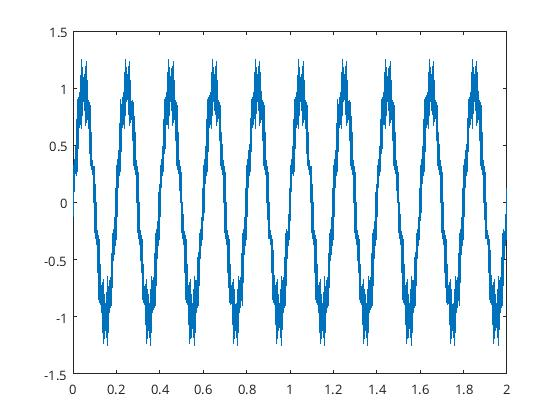
\includegraphics[width=.6\textwidth]{sin-noisy.jpg}
\caption{Quite the noisy sine sum function: $\sin (2\pi 5t) + 0.2 \cdot \sin (2\pi 200t) +  0.1 \cdot \sin (2 \pi 250t)$.}
\label{fig:sine-noisy}
\end{figure}

Looking at the signal in the frequency domain, we see the three main spikes corresponding to the three main components of the function (see Figure~\ref{fig:sin-noisy-fvtool}).

\begin{figure}[ht!]
\centering
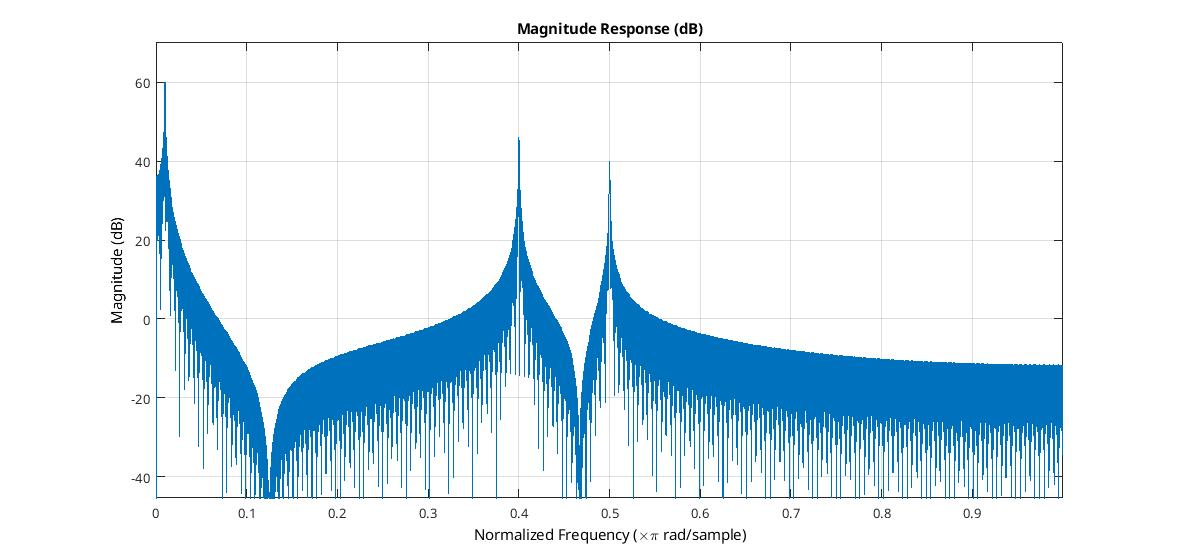
\includegraphics[width=.8\textwidth]{sin-noisy-fvtool.jpg}
\caption{Same noisy signal in the frequency domain (normalised).}
\label{fig:sin-noisy-fvtool}
\end{figure}

To clean the signal up, we can apply a low-pass filter that will only keep the main sine component. Let us design a simple Butterworth filter and apply on the signal:
\begin{minted}{matlab}
Bp = 500;       % Band-pass frequency
fs = 2*Bp;      % Sampling frequency
Wn = 0.1;       % Cut-off frequency
                % Wn must be 0.0 < Wn < 1.0, with 1.0 corresponding to half
                % the sample rate.
N = 10;         % Filter order
t = (0:1/fs:2);
x = sin(2*pi*5*t) + 0.2*sin(2*pi*200*t) + 0.1*sin(2*pi*250*t);
fvtool(x);
plot(t,x);
[b,a] = butter(N,Wn,'low');
fvtool(b,a);
xh = filter(b,a,x);
plot(t,xh);
\end{minted}

Figures~\ref{fig:butter-10} shows the filter profile and Figure~\ref{fig:sine-clean} the resulting signal, devoid of its noise.

\begin{figure}[ht!]
\centering
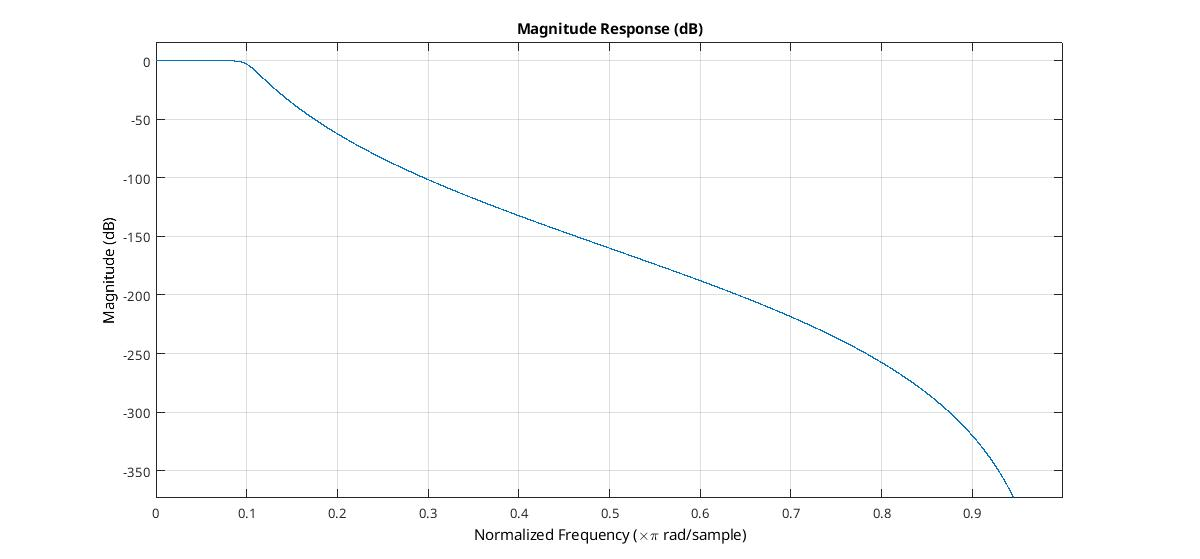
\includegraphics[width=.8\textwidth]{butter-10.jpg}
\caption{10-th order Butterworth low-pass filter.}
\label{fig:butter-10}
\end{figure}

\begin{figure}[ht!]
\centering
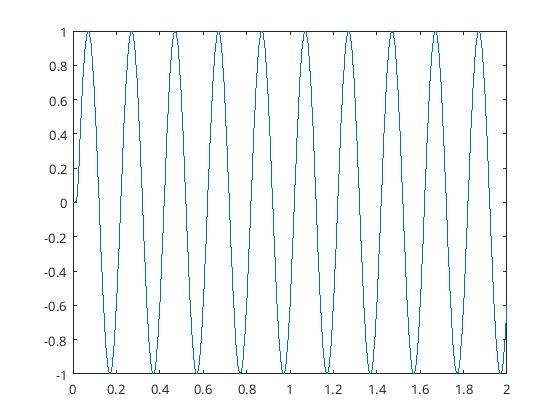
\includegraphics[width=.6\textwidth]{sin-clean.jpg}
\caption{Filtered signal.}
\label{fig:sine-clean}
\end{figure}


\begin{leftbar}
Play around with the filter order and the other types: Bessel (\texttt{besself}), Elliptic (\texttt{ellip}) and Chebyshev (\texttt{cheby1}).
Design a more complex input signal that can challenge your filters.
\end{leftbar}




Now if you wanted to do all this \textit{digitally}, it would need to be applied on a sampled, discretised signal and apply a convolution product between the signal and the filter.
If the product only needs past and present samples, this is effectively a Finite Impulse Response (FIR) filter. However if it displays a feedback loop and thus needs information ``from the future'', this is an Infinite Impulse Response (IIR) filter.
In this first part, we will focus on FIR filters.

If we investigate how the filtering should work, we get something like Figure~\ref{convol-product-ideal}.
$x(t)$ if the signal and $k'(t)$ is the filter.
This filter is a low-pass ``brick-wall'' filter, a perfect representation of what we would want.
After sampling, we obtain $x_e(t)$ and $k_e'(t)$. The both of them convoluted together\footnote{The magic of the convolution product is that it becomes a regular product in the frequency domain.} yield $y_e(t)$, where only the lower frequencies remain.

\begin{figure}[ht!]
\centering
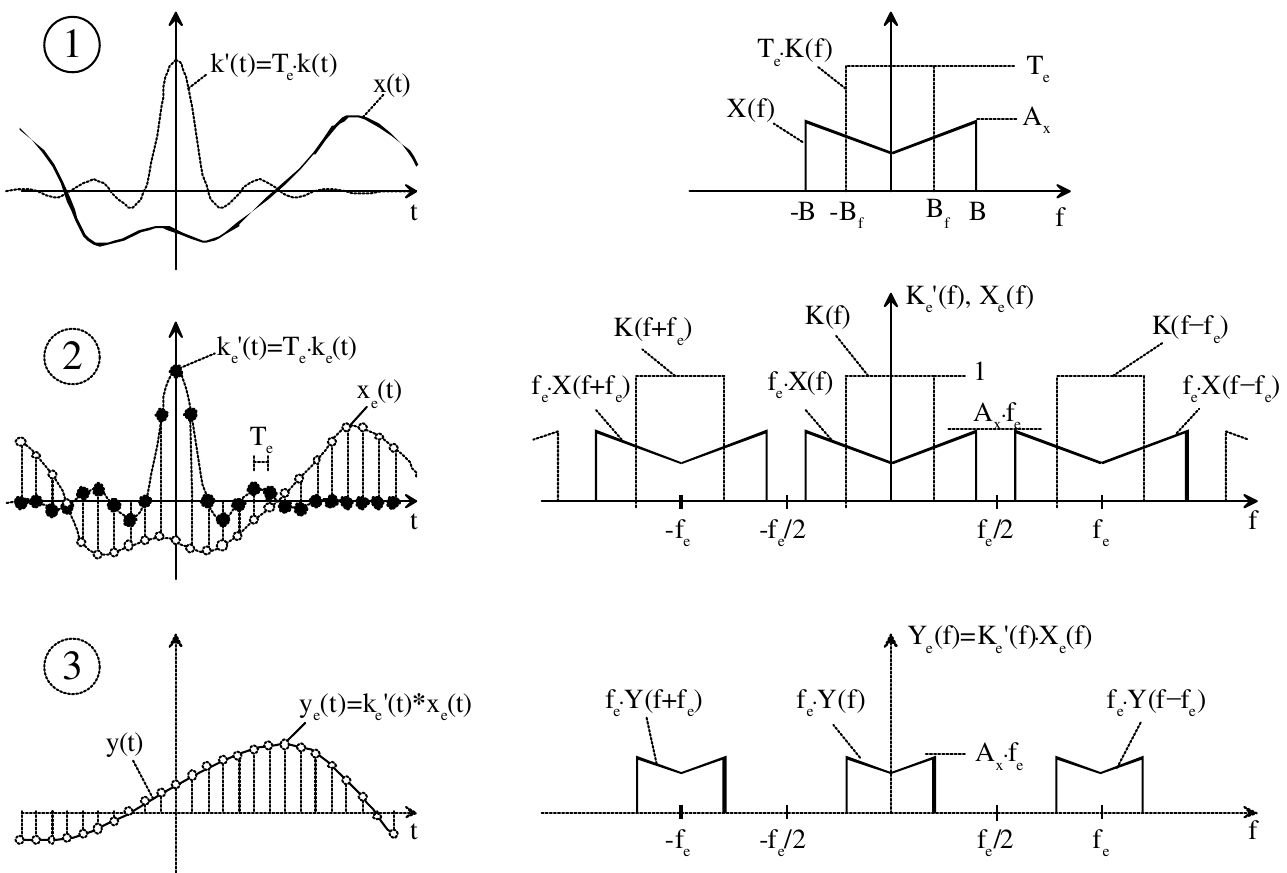
\includegraphics[width=\textwidth]{convol-product-ideal.png}
\caption{Time domain on the left, frequency domain on the right.}
\label{fig:convol-product-ideal}
\end{figure}

Sadly, our perfect brick-wall filter is not so easily represented in the time domain, as it needs an infinite time (both in the past and the future).
We thus need to do two things:
\begin{enumerate}
  \item Define the amount of values of the time domain filter we will keep. Those are referred as ``taps'' and represent the amount of coefficient that will need to be computed for each sample during the convolution product. The higher the amount of taps, the better, but the more resource intensive the computation becomes.
  The order $N$ of the resulting filter is directly linked to the amount of taps $N+1$.
  \item The type of ``windowing'' we will apply on the filter.
  We could perfectly say: ``I keep the $N+1$ taps as is and leave it be'', which would correspond to a rectangular window.
  Well, it actually turns out that is you bring the filter back into the frequency domain to analyse its shape at different frequencies, a rectangular window is not necessarily the best choice depending on the features you want for your filter.
  Do you want to have a low amplitude for the ripples in the passband or the stop-band? Or would you rather focus on the steepness of the transition between the two zones?
  Answering those questions is the art of FIR filter windowing.
\end{enumerate}


Hereunder follows a basic script to display and analyse a low-pass filter with an ideal rectangular window of order 20:
\begin{minted}{matlab}
N = 20; %Filter order
NbTaps = N+1;% Number of taps, i.e. points in the quantisation of the FIR filter
Bw = 1000; %1kHz bandwidth
fs = 4*Bw; %Sampling frequency
Wn = 2*Bw/fs; %Cut-off frequency
h_rect = fir1(N, Wn, 'low', rectwin(NbTaps), 'scale');
A = [1];
impz(h_rect, A); %Impulse response
figure;
freqz(h_rect, A); %Frequency analysis of both amplitude and phase
x = ones(NbTaps*2, 1); %Base signal with just ones
y = filter(h_rect, A, x); %Applies the above filter on the base signal
figure;
plot(y, 'b');
\end{minted}

\begin{leftbar}
Play around with the \texttt{fir1} function.

The filter type can take different values: \texttt{low}, \texttt{high}, \texttt{bandpass}, \texttt{stop}, \texttt{DC-0} or \texttt{DC-1}\footnote{\href{https://nl.mathworks.com/help/signal/ref/fir1.html\#bulla52-ftype}{matlab documentation}}.
Some of the main windowing functions are: \texttt{bartlett}, \texttt{chebwin}, \texttt{gausswin}, \texttt{hamming}, \texttt{hann}, \texttt{kaiser}, \texttt{rectwin} or \texttt{triang}\footnote{A full list is available in the \href{https://nl.mathworks.com/help/signal/referencelist.html?type=function&category=windows&s_tid=CRUX_topnav}{documentation}.}.
The main functions to use when doing spectrum analysis are: \texttt{freqz}, \texttt{impz}, \texttt{fvtools}.

Document your conclusions about the differences between the windowing functions.
\end{leftbar}




\section*{Assignment}
You are given a sample from a speech, but there are some noise superimposed\footnote{You can read and write audio using \texttt{audioread} and \texttt{audiowrite}.}.
Your task is to design a filter or a set of filters that will remove the unwanted components from the sample to restore it.
Start by analysing the audio sample in order to pinpoint the noisy parts of the signal.

You should upload your code and a 4 pages report to Claco by the due date indicated on the platform.

Evaluation criteria:
\begin{itemize}
  \item The report is clear and well written. (2 points)
  \item The source signal is clearly analysed and a relevant strategy is drawn. (2 points)
  \item The relative performance of each windowing function is highlighted through relevant figures in order to justify the choice made for the solution. (3 points)
  \item The filtering operation is performant and done efficiently, i.e. with low-order filters. It should thus be highlighted that a lower order filter would yield worse performance. (3 points)
  \item The report is in English. (1 bonus point)
\end{itemize}




\section*{Resource}
\begin{itemize}
	\item \href{https://www.mathworks.com/help/signal/referencelist.html?type=function&category=filter-design&s_tid=CRUX_topnav}{Filter design functions for \matlab}
  \item \href{https://octave.sourceforge.io/signal/overview.html}{Octave signal processing functions}
\end{itemize}


\end{document}
